\chapter{SYSTEM DESIGN AND ARCHITECTURE}

\section{System Overview}

TinkerBlocks is a comprehensive educational system that integrates multiple hardware and software components to create a seamless tangible programming experience. The system architecture follows a modular design approach, ensuring scalability, maintainability, and extensibility.

The system consists of four main components:
\begin{enumerate}
    \item \textbf{Programming Grid}: Physical board with camera for block recognition
    \item \textbf{Raspberry Pi Control System}: Central processing unit for computer vision and control
    \item \textbf{Robotic Car}: Programmable vehicle with sensors and actuators
    \item \textbf{Programming Blocks}: Physical blocks representing programming constructs
\end{enumerate}

\section{System Architecture}

The TinkerBlocks architecture consists of a three-layer design pattern:

\subsection{Core Layer}
The core layer provides foundational infrastructure with zero dependencies on other modules:
\begin{itemize}
    \item WebSocket server for real-time communication
    \item Process controller for workflow management
    \item Centralized configuration management
    \item Generic workflow execution framework
\end{itemize}

\subsection{Vision Layer}
The vision layer handles all computer vision and image processing tasks:
\begin{itemize}
    \item Image capture from camera systems
    \item Grid detection with perspective transformation
    \item OCR processing for text extraction
    \item Mapping of detected text to grid positions
\end{itemize}

\subsection{Engine Layer}
The engine layer implements the command interpreter and execution system:
\begin{itemize}
    \item Command parsing and validation
    \item Program execution with state management
    \item Variable and expression evaluation
    \item Control flow implementation (loops, conditionals)
\end{itemize}

\begin{figure}[H]
    \centering
    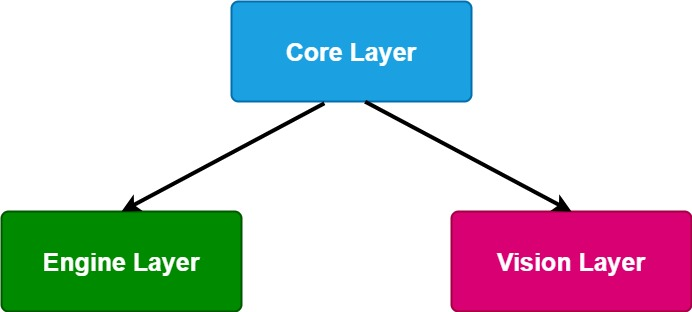
\includegraphics[width=0.8\textwidth]{assets/System_Arch.jpg}
    \caption{System Architecture}
    \label{fig:system_architecture}
\end{figure}

\section{Hardware Design}

\subsection{Robotic Car Specifications}

The robotic car serves as the primary execution platform for student programs. The design ensures precision, reliability, and educational value.

\subsubsection{Mechanical Design}
\begin{itemize}
    \item \textbf{Chassis}: Custom wooden frame (10cm × 20cm)
    \item \textbf{Propulsion}: Four DC motors with differential steering
    \item \textbf{Weight}: Approximately 500g 
    \item \textbf{Wheel Configuration}: Four-wheel drive
\end{itemize}

\subsubsection{Control Electronics}
\begin{itemize}
    \item \textbf{Main Controller}: Arduino Mega 2560 (primary control and sensor management)
    \item \textbf{WiFi Module}: ESP32 (wireless communication and API bridge)
    \item \textbf{Motor Drivers}: Two H-bridge modules for motor control
    \item \textbf{Power Management}: Voltage regulator (11.1V to 5V conversion)
\end{itemize}

\subsubsection{Sensor Integration}
\begin{itemize}
    \item \textbf{Navigation}: MPU-6050 gyroscope and accelerometer for precise orientation
    \item \textbf{Obstacle Detection}: HC-SR04 ultrasonic sensor (front-mounted)
    \item \textbf{Line Detection}: Two IR sensors for path boundary detection
    \item \textbf{Drawing Mechanism}: Servo-controlled pen for drawing operations
\end{itemize}

\subsubsection{Power System}
\begin{itemize}
    \item \textbf{Battery Pack}: Three 3.7V lithium-ion batteries (11.1V total)
    \item \textbf{Operating Time}: Approximately 2-3 hours of continuous operation
    \item \textbf{Charging}: External charging system with safety protection
\end{itemize}

\subsection{Programming Grid Board}

The programming grid serves as the interface for arranging programming blocks and capturing their configuration.

\subsubsection{Physical Structure}
\begin{itemize}
    \item \textbf{Grid Size}: 16 columns × 10 rows (configurable)
    \item \textbf{Block Placement}:  drag and drop by hand into holes.
    \item \textbf{Material}: wood construction (PVC)
    \item \textbf{Portability}: Lightweight design for classroom use
\end{itemize}

\subsubsection{Camera System (OAK-D)}
\begin{itemize}
    \item \textbf{Position}: Overhead mounting for full grid visibility
    \item \textbf{Resolution}: High-resolution camera for accurate text recognition
    \item \textbf{Lighting}: Controlled lighting conditions for consistent image quality
    \item \textbf{Calibration}: Automated corner detection and perspective correction
\end{itemize}

\subsection{Control Station}

The Raspberry Pi-based control station manages the entire system operation.

\subsubsection{Hardware Specifications}
\begin{itemize}
    \item \textbf{Processor}: Raspberry Pi 4 (2GB RAM)
    \item \textbf{Storage}: 32GB microSD card for system and data storage
    \item \textbf{Display}: Tablet for status and game mode information
    \item \textbf{Input}: Buttons and Applcation on Tablet for user interaction
    \item \textbf{Connectivity}: WiFi for car communication, USB for camera
\end{itemize}

\section{Software Architecture}

\subsection{Modular Design Principles}

The software architecture follows clean architecture principles with clear separation of concerns:

\begin{itemize}
    \item \textbf{Dependency Inversion}: Core modules have zero dependencies on implementation details
    \item \textbf{Protocol-Based Design}: Interfaces defined through Python protocols for extensibility
    \item \textbf{Async-First Architecture}: Built on asyncio for concurrent operations
    \item \textbf{Workflow Pattern}: Generic execution framework supporting cancellation and chaining
\end{itemize}

\subsection{Communication Architecture}

The system implements a multi-protocol communication architecture:

\subsubsection{WebSocket Communication}
\begin{itemize}
    \item Real-time bidirectional communication between components
    \item JSON-based message protocol for command and status exchange
    \item Broadcast support for multiple client connections
    \item Connection management with automatic reconnection
\end{itemize}

\subsubsection{Serial Communication}
\begin{itemize}
    \item Arduino-ESP32 communication via UART (115200 baud)
    \item Command-response protocol with JSON payloads
    \item Error handling and timeout management
    \item Flow control for reliable data transmission
\end{itemize}

\subsubsection{HTTP API}
\begin{itemize}
    \item RESTful API exposed by ESP32 for car control
    \item Stateless design for reliable remote operation
    \item JSON request/response format for all endpoints
    \item Error reporting with appropriate HTTP status codes
\end{itemize}

\section{Programming Language Design}

\subsection{Visual Programming Constructs}

The TinkerBlocks programming language supports fundamental programming concepts through physical blocks:

\subsubsection{Movement Commands}
\begin{itemize}
    \item \textbf{MOVE}: Forward/backward movement with distance parameters
    \item \textbf{TURN}: Left/right rotation with angle specifications
    \item \textbf{WAIT}: Pause execution for specified time duration
\end{itemize}

\subsubsection{Control Flow}
\begin{itemize}
    \item \textbf{LOOP}: Repetition with count or conditional parameters
    \item \textbf{IF/ELSE}: Conditional execution based on sensor inputs
    \item \textbf{WHILE}: Conditional loops with real-time evaluation
\end{itemize}

\subsubsection{Data Manipulation}
\begin{itemize}
    \item \textbf{SET}: Variable assignment and arithmetic operations
    \item \textbf{Variables}: Named storage for numeric and boolean values
    \item \textbf{Expressions}: Mathematical and logical operations
\end{itemize}

\subsubsection{Input/Output}
\begin{itemize}
    \item \textbf{PEN\_UP/PEN\_DOWN}: Drawing control for creative tasks
    \item \textbf{Sensor Values}: Distance, obstacle detection, line sensing
    \item \textbf{Boolean Operations}: Logical combinations of conditions
\end{itemize}

\subsection{Syntax and Semantics}

The visual programming language uses indentation-based syntax similar to Python:

\begin{itemize}
    \item \textbf{Block Arrangement}: Left-to-right, top-to-bottom reading order
    \item \textbf{Indentation}: Column position determines nesting level

\end{itemize}



\section{User Interface Design}

\subsection{Physical Interface}

The system provides intuitive physical interaction through:

\begin{itemize}
    \item \textbf{Block Placement}: mechanical guides for precise positioning
    \item \textbf{Visual Feedback}: Real-Time updates sending to an app.
    \item \textbf{Control Buttons}: Start, stop buttons
    \item \textbf{Display Screen}: a Mobile Screen with App running on it.
\end{itemize}

\subsection{Digital Interface}

\subsubsection{Monitoring}
\begin{itemize}
    \item camera feed showing current block arrangement
    \item Program execution visualization with updates sending to app
\end{itemize}

\subsubsection{Educational Features}
\begin{itemize}
    \item Step-by-step program execution with optional pauses
    \item Error messages with educational explanations
\end{itemize}

\section{Scalability and Extensibility}

\subsection{Hardware Scalability}

The modular hardware design supports future extensions:

\begin{itemize}
    \item \textbf{Additional Sensors}: Expandable I/O for new sensor types
    \item \textbf{Multiple Cars}: Support for multi-robot scenarios
    \item \textbf{Larger Grids}: Scalable grid sizes for complex programs
    \item \textbf{Enhanced Actuators}: Additional output devices (speakers, lights)
\end{itemize}

\subsection{Software Extensibility}

The software architecture enables easy extension:

\begin{itemize}
    \item \textbf{Command Registry}: Plugin-style command addition
    \item \textbf{Workflow Framework}: Generic execution patterns
    \item \textbf{Protocol Abstraction}: Support for different communication methods
    \item \textbf{ِAI}: Support for AI coding like Github-copilot
\end{itemize}

\section{Performance Requirements}

\subsection{Real-time Performance}

The system is designed to meet specific performance criteria:

\begin{itemize}
    \item \textbf{Image Processing}: Block recognition within 2 seconds
    \item \textbf{Program Execution}: Immediate response to program start
    \item \textbf{Car Control}: Sub-100ms latency for movement commands
\end{itemize}



This comprehensive design provides a solid foundation for implementing an effective educational robotics system that combines the benefits of tangible programming with modern robotics technologies.